%----------------------------------------------------------------------------------------
%	PACKETS AND CONFIGURATION
%----------------------------------------------------------------------------------------

\documentclass[11pt]{beamer}
\setbeamercovered{transparent}

\usepackage{title}  		% Title settings for the presentation
\usepackage{parskip}    	% Paragraph indent & skip
\usepackage{xcolor}     	% More colors
\usepackage{enumitem}		% Better lists
\usepackage{graphicx}  		% 'graphics' package interface
\usepackage{listings}   	% Code sections formatting}
%\usepackage{pdftexcmds}
%\usepackage{minted}
%\usepackage[utf8]{inputenc}
%\usepackage[T1]{fontenc}
%\usepackage{pythontex}
\usepackage{verbatim}

% Custom colors
\definecolor{AnnotationGreen}{RGB}{34, 128, 45}
\definecolor{CommentGreen}{RGB}{29, 204, 49}

% Python code formatting
% Use it by creating an environment like \begin{lstlisting}[style=Python] ... \end{lstlisting}
% Since annotations aren't tagged as keywords I have inserted a manual delimiter for them,
% it works as follows: \@@AnnotationText@@/
\lstdefinestyle{Python}{
    language = Python,
    basicstyle = \footnotesize\ttfamily,
    commentstyle = \textcolor{CommentGreen},
    stringstyle = \textcolor{orange},
    showstringspaces = false,
    keywordstyle = \textcolor{blue},
    moredelim = [is][\textcolor{AnnotationGreen}]{\\@}{@@\/},   % Annotations
    numberstyle = \scriptsize\ttfamily\textcolor{gray},
    numbers = left,
    frame = single,
    frameround = tttt,
    framexleftmargin = 10pt,
    framexrightmargin = 0pt
}

% HELPER PACKAGES (TODO: REMOVE IN FINAL) %
\usepackage{todonotes}
\presetkeys{todonotes}{inline}{}
\usepackage{blindtext}
%\usepackage{amsmath} %math packages dunno if is the best.
% HELPER PACKAGES (TODO: REMOVE IN FINAL) %

\usetheme{Copenhagen} % THEME

%----------------------------------------------------------------------------------------
%	DOCUMENT
%----------------------------------------------------------------------------------------

\begin{document}

% TITLE
\frame{\titlepage}

% Table of Contents
\begin{frame}{Project}
    \tableofcontents[hideallsubsections]
\end{frame}

% Environment and Simulation ------------------------------------------------------------

\AtBeginSection[]
{
\begin{frame}{}
    \tableofcontents[sections={\thesection}]
\end{frame}
}

% ----------------------------------------

\section{Introduction}

%-----------------------------------------

\begin{frame}

\frametitle{Introduction}
\framesubtitle{Project scope}

The focus of this project is to optimize the budget allocated for the advertisement campaigns of 5 different items in order to maximize the profit of an e-commerce website that sells products to the public.
Each page has a primary product and some secondary products, each user that lands on a page has a possibility to buy the primary prodcut and/or proceed to one of the secondaries with a given probability, the process repeats.

\end{frame}


%-----------------------------------------

\begin{frame}

\frametitle{Introduction}
\framesubtitle{Project scope}

The optimization has to be perfomed on different scenarios and different algorithms.
We had to direct our focus on bandit algorithms combining Gaussian Process with Upper Confidence Bound and Thompson Sampling algorithms.
For each different scenario the performance of the learners based on these algorithm is evaluated against the Clayrvoiant and the Stupid Learner.

\end{frame}

%-----------------------------------------

\begin{frame}

\frametitle{Introduction}
\framesubtitle{General hypoteses}

The main general hypoteses that were given to us are:
\begin{itemize}[label={-}]
    \item For every primary product, the secondary products to display and their order is fixed.
    \item The price of every product is fixed and it is equal to the margin.
    \item By clicking a specific ad, the user lands on the corresponding primary product.
\end{itemize}

\end{frame}

% ----------------------------------------

\section{Environment and Simulator}

%-----------------------------------------

\subsection{Overview}

%-----------------------------------------

\begin{frame}

\frametitle{Environment and Simulator}
\framesubtitle{General hypotesis}

For this project, we are required to design an Environment that satisfies various constraints both on the e-commerce site's properties and on the users' behavior; in addition, since most of the tasks were generic, we had to come up with some of our own assumptions.
In particular we want to underline the following for the e-commerce website:
\begin{itemize}[label={-}]
    \item The website has unlimited units for the 5 different items.
    \item Actions on the webpages are perfectly observable by the ecommerce website.
\end{itemize}

\end{frame}

% ----------------------------------------

\begin{frame}

\frametitle{Environment and Simulator}
\framesubtitle{General hypotesis}

...and we assume that the users present the following behaviors:
\begin{itemize}[label={-}]
    \item Every day, there is a random number (subject to noise) of potential new users.
    \item The reservation price for each user is always over the single unit.
    \item The users can activate parallel paths while on the webpage.
    \item The number of items that a user will buy is a random variable, independent from any other variable.
\end{itemize}

\todo{insert text somewhere}
%The behavior of a user is modelled as a graph where nodes represent product pages and weights represent the probabilities for the user to click from the primary item of the page to one of the secondaries.

\end{frame}

%-----------------------------------------

\subsection{Environment structure}

%-----------------------------------------

\begin{frame}[fragile]

\frametitle{Environment and Simulator}
\framesubtitle{Environment}

The environment is modelled as a python dataclass containing the following attributes:

\begin{lstlisting}[style=Python, basicstyle=\tiny, numbers=none, framexrightmargin=-20pt]
    # The total budget to subdivide
    total_budget: int

    # Probability of every class to show up. They must add up to 1
    class_ratios: List[float]

    # Features associated to every class
    class_features: List[List]

    # Price of the 5 products
    product_prices: List[float]

    # List of class parameters for each class and product,
    # implemented as list of lists of UserClassParameters.
    # Each class has distinct parameters for every product
    classes_parameters: List[List[UserClassParameters]]
\end{lstlisting}

\end{frame}

% ----------------------------------------

\begin{frame}[fragile]

\frametitle{Environment and Simulator}
\framesubtitle{User classes}

We modelled the $\alpha$-functions, which compute the expected value of interactions on a product given a fixed budget, as exponential functions.
In particular their upper bound represents the maximum expected number of interactions possible while the maximum useful budget isthe amount of budget after which any budget increase would not lead to a ratio increase.


\begin{lstlisting}[style=Python, basicstyle=\tiny, numbers=none, framexrightmargin=-20pt]
    # Lambda parameter, which is the probability of osserving the
    # next secondary product according to the project's assignment
    lam: float

    # Max number of items a customer can buy of a certain product.
    # The number of bought items is determined randomly with
    # max_items as upper bound
    max_items: int

    # Products graph's matrix. It's a empty matrix, should be
    # initialized with populate_graphs
    graph: np.ndarray

    # List that constains for every i+1 product the secondary i+1
    # products that will be shown in the first and second slot
    next_products: List[Tuple[int, int]]

    # Controls randomness of the environment
    random_noise: float
\end{lstlisting}

\end{frame}

% ----------------------------------------

\begin{frame}

\frametitle{Environment and Simulator}
\framesubtitle{User classes}

\begin{itemize}[leftmargin=*, label={$\circ$}]
    \item Users are subdivided in classes based on their 2 binary features for a total of 3 different classes.
    \item In particular, each user class is defined by its $\alpha$-functions (one for each product plus the one for the non-strategic competitor) which define the probability of landing on a given product page.
    \item Each $\alpha$-function is defined by the values: \textbf{reservation price}, \textbf{upper bound} and \textbf{maximum useful budget}
\end{itemize}

\todo{alpha functions aren't sigmoidal! we changed to the exponential function - correct and move to a new slide maybe}
%Since the $\alpha$-functions we had choosen belong to the sigmoidal class we need these additional parameters.
%\begin{figure}[⟨r⟩]
%\includegraphics[height=3.8cm]{img/Graphs/exponential.png}
%\end{figure}

\end{frame}

% ----------------------------------------

\begin{frame}

\frametitle{Environment and Simulator}
\framesubtitle{Masked Environment}

Alongside the Environment we define a Masked Environment with the purpose of hiding crucial information to the learners since each type of learner should only have access to a subset of all the information available in the environment dictated by the type of learner.

The masked environment isn't strictly needed in the project since the learners could easily ignore the extra information, however, we wanted to face the problem with an approach aimed towards reusability and extendability and in this case (as in many others down the line) we opted for a more generalizable solution.

\todo{we talk about learners without metioning them before, we need to introduce them in the introductory section}

\end{frame}

% ----------------------------------------

\subsection{Randomness in the Environment}

% ----------------------------------------

\begin{frame}

\frametitle{Environment and Simulator}
\framesubtitle{Randomness in the Environment}

\begin{itemize}[leftmargin=*, label={$\circ$}]
    \item For the sake of representing a real scenario, most of the values that are not known a priori are randomly generated and every variable that evolves through time without our direct control has elements of randomness to it (for instance, each day we randomly get the number of active total users in our scenario by using a gaussian distribution with tunable mean and standard deviation).
    \item Even though most of the randomness is tunable and controlled through seeded generators, there are still impactful elements of non determinism (i.e. the Dirichlet distribution) that are not possible to control in any way.
\end{itemize}

\end{frame}

% ----------------------------------------

\begin{frame}

\frametitle{Environment and Simulator}
\framesubtitle{Example of Environment}

We see here an example of environment initialization:
\todo{improve legibility}


%\begin{figure}[<t>]
%   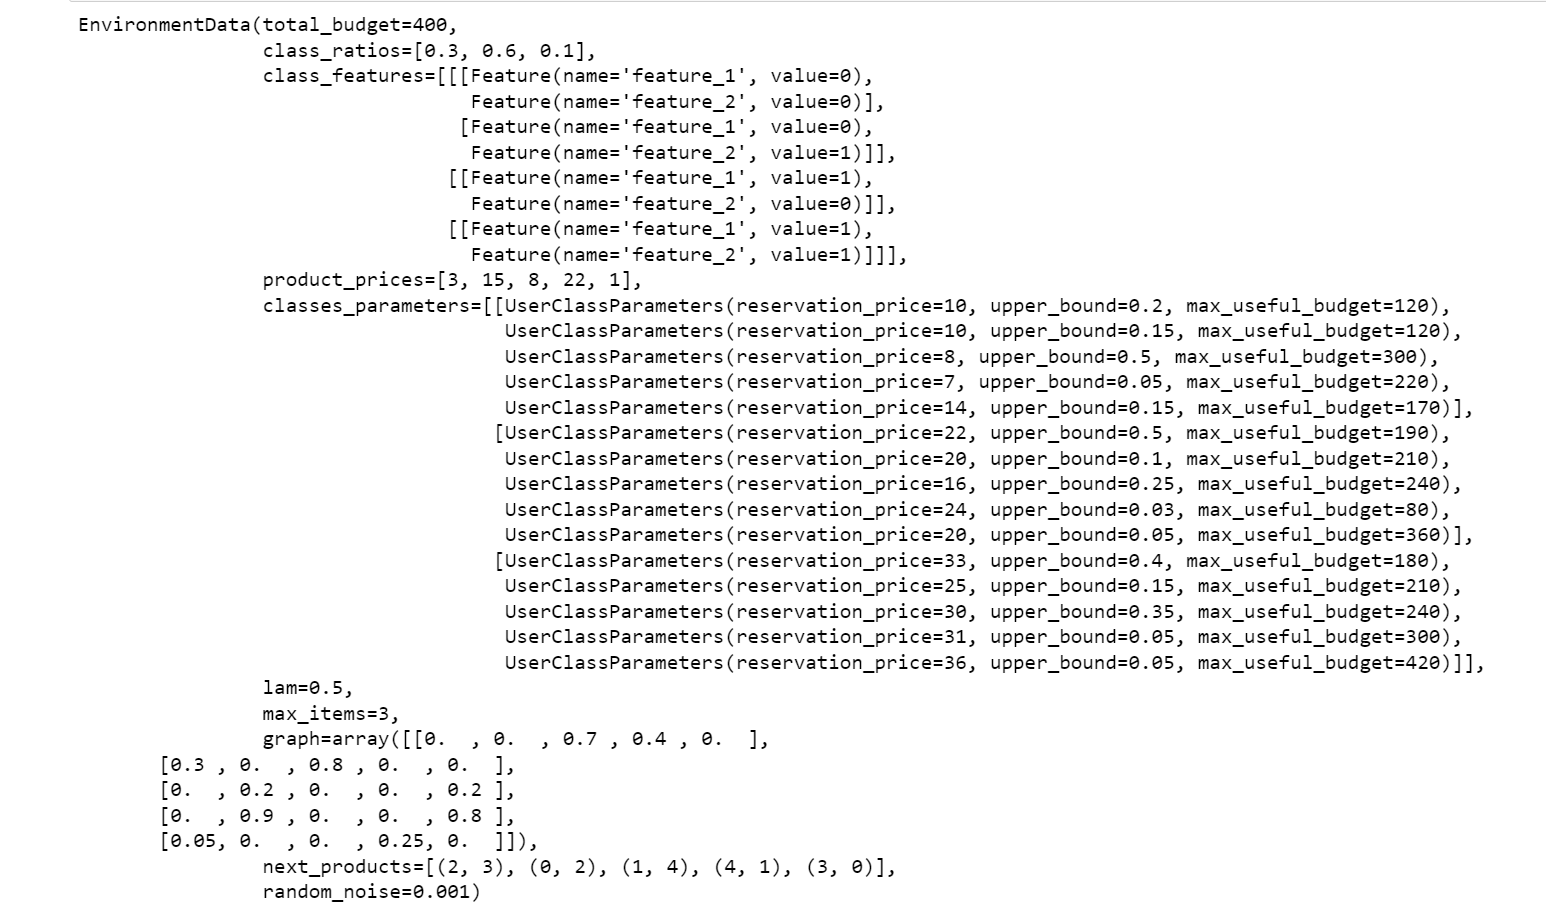
\includegraphics[height=6cm]{img/Graphs/Example_environment.png}
%\end{figure}

\end{frame}

% ----------------------------------------

\subsection{Simulation}

% ----------------------------------------

\begin{frame}

\frametitle{Environment and Simulator}
\framesubtitle{Daily Simulation}

\begin{itemize}[leftmargin=*, label={$\circ$}]
    \item The Simulation class is the main engine that brings together learner and environment by making them interact with each other while offering an interface to customize the execution.
    \item The basic idea of the simulation is to simulate a real scenario day by day using the environment to generate interactions with the website according to the budgets that the current learner proposed and then, feed the results back to the learner to make it actually learn.
    \item Repeating the simulation execution step for each day until an arbitrary time horizon is reached grants us all the data needed to evaluate the performance of our learner.
\end{itemize}

\end{frame}

% ----------------------------------------

\begin{frame}

\frametitle{Environment and Simulator}
\framesubtitle{Daily Simulation}

\todo{insert generic learner execution plot over n days}

\end{frame}

% Optimization Algorithm ----------------------------------------------------------------

\AtBeginSection[]
{
\begin{frame}{}
    \tableofcontents[sections={\thesection}]
\end{frame}
}

% ----------------------------------------

\section{Optimization Algorithm}

% ----------------------------------------

\subsection{General Problem}

% ----------------------------------------

\begin{frame}

\frametitle{Optimization Algorithm}
\framesubtitle{Problem Formulation}

The purpose of the optimization algorithm is to find the optimal budget for each campaign in order to maximize the profit, which is defined as the difference between the profits gained from selling products and the advertisement expenses.
Basically, it is the maximization problem subject to an obvious constraint: the sum of the daily budget can't be greater then the overall budget.

The optimization problem can be expressed as follows:
\begin{displaymath}
F=\max_{\substack{x_i\in B}} \sum_{i=0}^n \alpha_i(x_i)p_i-x_i \ s.t. \sum_{i=0}^n x_i\leq B
\end{displaymath}

\end{frame}

% ----------------------------------------

\subsection{Algorithm}


\begin{frame}

\frametitle{Optimization Algorithm}
\framesubtitle{}
\todo{talking about the code in words}

\end{frame}

% ----------------------------------------

\begin{frame}

\frametitle{Optimization Algorithm}
\framesubtitle{}
\todo{snippets of code}

\end{frame}

% Uncertain alpha functions -------------------------------------------------------------

\AtBeginSection[]
{
\begin{frame}{}
    \tableofcontents[sections={\thesection}]
\end{frame}
}

% ----------------------------------------

\section{Uncertain $\alpha$-functions}

% ----------------------------------------

\subsection{General Approach}

% ----------------------------------------

\begin{frame}

\frametitle{Uncertain $\alpha$-functions}
\framesubtitle{General Approach}

In order for our project to have a more general outline, we decided to model a generic Learner interface to standardize how our agents should be expected to behave while learning the budget distribution for a set of subcampaigns in a specific scenario defined by the environment.

In particular, each Learner is characterized by the \textit{learn} and \textit{predict} actions.
Every different type of learner will also receive a customized set of information filtered by the masked enviroment (in line with each project step) and potentially employs different algorithms to learn and predict the various budgets.

\end{frame}

% ----------------------------------------

\begin{frame}[fragile]

\frametitle{Uncertain $\alpha$-functions}
\framesubtitle{General Approach}

%
%Arguments: interactions: the interactions of the users which led to the given reward reward: the reward obtained from the environment based on the prediction given, needed for the tuning of internal properties done by the learner
%prediction: array containing the previous budget evaluation of the learner
%
%Arguments: data: up-to-date, complete or incomplete environment information that is used by the learner in order to make the inference
%Returns: a tuple containing a list of values (corresponding to the budgets inferred given the knowledge obtained by the learner until now) and a list of features (referring to which particular customers were the budgets aimed for, if None, the budgets apply to all the customers)



\begin{lstlisting}[style=Python, basicstyle=\tiny, numbers=none, framexrightmargin=-20pt]
class Learner(ABC):

#Updates the learner's properties according to the reward received.
@abstractmethod
def     learn(self, interactions: List[Interaction], reward: float,
             prediction: np.ndarray):
 pass

 #Makes an inference about the values of the budgets for the subcampaigns
 #from the information got over time and the current environment

@abstractmethod 
def     predict(self, data: MaskedEnvironmentData) -> 
        Tuple[np.ndarray, Optional[List[List[Feature]]]]: 
pass

#Creates a figure and plots showing the status of learning progress
@abstractmethod 
def     show_progress(self, fig: plt.Figure):
pass
    
\end{lstlisting}

\end{frame}

% ----------------------------------------

\begin{frame}

\frametitle{Uncertain $\alpha$-functions}
\framesubtitle{General Approach}

Both Thompson Sampling (TS) and Upper Confidence Bound (UCB, in particular UCB1), in conjunction with Gaussian Processes are the algorithms chosen for the learners to use.

\todo{insert TS formulations}

\end{frame}

% ----------------------------------------

\begin{frame}

\frametitle{General Approach}
\framesubtitle{UCB1 formulation}

In this algorithm, every arm is associated with an upper confidence bound which provides an estimation of the reward provided by playing that arm.
Then, after have played all arms to have an indication of thier reward, at every trial the arm, with the highest upper confidence bound, is picked (optimism in the face of uncertainty).
After having collected the realization of the reward of the chosen arm, the upper confidence bound is updated.


\end{frame}

% ----------------------------------------

\begin{frame} [fragile]

\frametitle{General Approach}
\framesubtitle{UCB1 formulation}

The main peculiarity combining gaussian process with UCB1 is that is possible to take advantage of the GP's confidence interval and modeling it as a confidence bound.

\begin{lstlisting}[style=Python, basicstyle=\tiny, numbers=none, framexrightmargin=-20pt]
def estimation(self):
upper_bounds = (self.means + self.confidence * 1.96 * self.sigmas)
                 * self.normalize_factor
return upper_bounds

\end{lstlisting}

The theoretical regret given by this kind of algorithm is buonded by:

\begin{displaymath}
  P(UCB1) \le  \sum_{a:\mu_a < \mu_a^*} \frac{4log(T)}{\Delta_a} + 8\Delta_a 
\end{displaymath}
where $\Delta_a$ is the difference in expected reward between the optimal arm $a^*$ and the arm $a$

\todo{fix edges(probably no need code)}

\end{frame}

% ----------------------------------------

\begin{frame}

\frametitle{General Approach}
\framesubtitle{TS formulation}

Some aspect are similar to the UCB1 since both belong to the bandit algorithm the main difference is that here to every arm is associated a prior distribution.
Every arm has a prior on its expected value based on his mean distribution.
After drawing a sample according to the corresponding prior distribution, the algorithm choose the arm with the best sample (optimism in the face of uncertainty).
Then it updates the distribution of the chosen arm according the observed realization

\end{frame}

% ----------------------------------------

\begin{frame}[fragile]

\frametitle{General Approach}
\framesubtitle{TS formulation}

The implementation of the Gaussian Process combining Tomphson Sampling algorithm is used to fit and estimate a function using a gaussian process and normal distributions
The theoretical regret given by this kind of algorithm is buonded by:
\begin{displaymath}
  %  P(TS) \le (1+\epsilon) \sum_{a:\mu_a < \mu_a^*} \frac{\Delta_a(log(T)+log(log(T)))}{K*\Lambda(mu_a*,mu_a)} + C (\epsilon, \mu_a1 , ... , \mu_a_\left|A\right|)  
\end{displaymath}
where $K*\Lambda(mu_a*,mu_a)$ is the Kullback-Leibler divergence and as before $\Delta_a$ is defiened as the difference in expected reward between the optimal arm $a^*$ and the arm $a$
\todo{non capisco dove sia l'errore nella formula}
\end{frame}

% ----------------------------------------

\begin{frame}

\frametitle{General Approach}
\framesubtitle{Comparing results}

For each different learner, when possible, we will show our results through the comparison of the rewards obtained by each algorithm against the rewards achieved (in the same enviroment setting) from the Clairvoyant learner and the Stupid learner.
This, aside from theoretical formulations, will help us to define upper bounds and lower bounds for different solutions.


\end{frame}

% ----------------------------------------

\begin{frame}

\frametitle{General Approach}
\framesubtitle{Comparing results}

In particular the Clayrvoiant Learner learn and predict on complete dataset available, de facto solving the optimization problem as at each time while the "stupid" one always subdivides equally the budget between products and
doesn't update its prediction.

\todo{this two slides repeat a lot without adding much, we need to move this part in the Introduction and merge this with the slide that already talks about this. i agree i was actually thinking this all sub section could ahve be placed somewhere in the Introduction or after the optimization problem}
\end{frame}

%----------------------------------------

\subsection{Contextual hypotesis}

% ----------------------------------------

\begin{frame}

\frametitle{Uncertain $\alpha$-functions}
\framesubtitle{Scenario}

We now assume that the binary features of the users cannot be observed and therefore user are aggregated by class.
Since the features of the users are \textbf{not observable}, the alpha functions' shape of each class is unknown. 
the algorithm receives all the interactions minus the parameters of the alpha fucntions.

\end{frame}

% ----------------------------------------

\subsection{Algorithm}

% ----------------------------------------

\begin{frame}

\frametitle{Uncertain $\alpha$-functions}
\framesubtitle{Algorithm}

\todo{how do we solve the problem}
First of all through the Masked Environment the Learner receive only the appropriate set of data.
Our Alphaless Learner creates 5 different GP-Learner one for each product which exploit the TS and UCB1 algorithm seen before.
\todo{how the algorithm works}
They learn and predict on the aggregated budget matrix and try to find the optimal allocation of the budget.
It is also adapted, if need, to have a sliding window in order to better perform in a varing environment.

\end{frame}

% ----------------------------------------

\subsection{Results}

%-----------------------------------------

\begin{frame}

\frametitle{Uncertain $\alpha$-functions}
\framesubtitle{Results}
\todo{code snippet (if needed)}
\todo{insert some graph of performance vs clayrvoiant vs stupid}

\end{frame}

%-------------------------------------------

\AtBeginSection[]
{
\begin{frame}{}
    \tableofcontents[sections={\thesection}]
\end{frame}
}

% Uncertain alpha functions and number of items sold ------------------------------------

\section{Uncertain $\alpha$-functions and number of items sold}

%-----------------------------------------

\subsection{Contextual hypotesis}

%-----------------------------------------

\begin{frame}

\frametitle{Uncertain $\alpha$-functions and Units sold}
\framesubtitle{Scenario}

In this case the ecommerce doesn't register either the units sold of each products and the class parameters.
The learner will receive aggregated data so it must work by estimating aggregated alpha functions and it estimates the reward given by every single product.

\end{frame}

%---------------------------------------------

\subsection{Algorithm}

%---------------------------------------------

\begin{frame}

\frametitle{Uncertain $\alpha$-functions and Units sold}
\framesubtitle{Algorithm}

This learner try to optimize from the list of interactions but recieve only the aggreagated data.
so in order to work it estimate the list of values, corresponding to the earnings for each product given the knowledge obtained by the learner until now
We separately consider all the aggregated interactions where users landed on a certain product, then compute the reward they generated.
This way we obtain reward associated to a single campaign.
 \todo{devo capire cose e riscrivere.}

\end{frame}

% ----------------------------------------

\subsection{Results}

%-----------------------------------------

\begin{frame}

    \frametitle{Uncertain $\alpha$-functions and Units sold}
    \framesubtitle{Results}

    \todo{insert performance graph}

\end{frame}

% ----------------------------------------

% Uncertain graph weights ---------------------------------------------------------------

%\section{Uncertain Graph Weights}

% Non-stationary demand curve -----------------------------------------------------------

%\section{Non-stationary demand curve}

% Context generation --------------------------------------------------------------------

%\section{Context generation}

\end{document}


%NOTE TO US:
%%\centering if we want the presentation to be power-point style
